% # COPYRIGHT:
%
% Copyright (C) 2011 Jeremiah Mahler <jmmahler@gmail.com>.
% Permission is granted to copy, distribute and/or modify this document
% under the terms of the GNU Free Documentation License, Version 1.3
% or any later version published by the Free Software Foundation;
% with no Invariant Sections, no Front-Cover Texts, and no Back-Cover Texts.
% A copy of the license is included in the file "fdl-1.3.txt".
%
\documentclass[12pt]{article}
%\usepackage{mslapa}
\usepackage{hyperref}
\usepackage{amsmath}
\usepackage{graphicx}
\usepackage{ulem}
\usepackage{vmargin}
\usepackage{tabularx}
\usepackage{sectsty}
\usepackage{pbox}
\usepackage{bigstrut}
\usepackage{enumerate}
\usepackage{parskip} % add spaces between paragraphs
\input kvmacros % Karnaugh Maps and Veitch charts
%\usepackage{cleveref}
\usepackage{verbatim}
\usepackage{listings}

\setpapersize{USletter}
\setmarginsrb{1.0in}{1.0in}{1.0in}{1.0in}{0in}{0.25in}{0in}{0.20in}

\sectionfont{\normalsize}
\subsectionfont{\normalsize}

% configure \bigstrut size
% This configures spacing above and below rows in a tabularx.
%\renewcommand{\bigstrutjot}{6pt}

\renewcommand{\bigstrutjot}{2.0\jot}

\setlength{\parindent}{0in}

\raggedright

\begin{document}

% {{{ Cover Page
\centerline{\bf EECE 144}
\centerline{\bf Fall 2011}
\centerline{\bf}
\centerline{\bf Lab Report \#13}
\centerline{\bf Section 4}
\centerline{\bf 12/07/2011} % date due
% signature area
\begin{center}
\begin{tabularx}{\textwidth}[b]{X l l}
Submitted by: Jeremiah Mahler & & \\
Signature & Printed Name & Date \\
\hline
\multicolumn{1}{|X|}{} & \multicolumn{1}{|l|}{\bigstrut \bf Jeremiah Mahler} & \multicolumn{1}{|l|}{\bf Dec 7, 2011} \\
\hline
\multicolumn{1}{|X|}{} & \multicolumn{1}{|l|}{\bigstrut \bf Marvanee Johnson} & \multicolumn{1}{|l|}{\bf Dec 7, 2011} \\
\hline
\end{tabularx}
\end{center}
% }}}

% {{{ Description/Objectives
\section{Description/Objectives}

The goal of this lab is to design a circuit in Verilog\cite{VERILOG}
which replicates the tail light operation of an older model Thunderbird.

\begin{quote}
\begin{center}
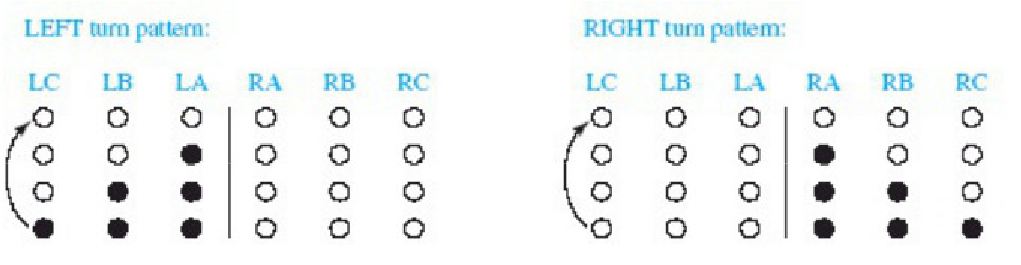
\includegraphics[scale=0.7]{thunderbird-lights}
\end{center}

Design a Moore sequential circuit to control these lights.
The circuit has three inputs LEFT, RIGHT and HAZ.  LEFT and
RIGHT come from the driver's turn signal switch and cannot be 1 at the same
time.
As indicated above, when LEFT = 1 the lights flash in a pattern LA on;
LA and LB on; LA, LB, and LC on; all off; and then the sequence repeats.
When RIGHT = 1, the light sequence is similar.
If a switch from LEFT to RIGHT (or vice versa) occurs in the middle of a flashing
sequence, the circuit should immediately go to the IDLE (lights off) state
and then, start the new sequence.  HAZ comes from the hazard switch,
and when HAZ = 1, all six lights flash on and off in unison.
HAZ takes precedence if LEFT or RIGHT is also on.
Assume that a clock signal is available with a frequency equal to the desired
flashing rate.
\end{quote}
\cite[p. 547, prob. 16.27]{roth2009fundamentals}.

% }}}

% {{{ Procedure
\section{Procedure}
\label{sec:procedure}

There is more than one way to design this circuit.
The method used here builds a state diagram and state table
for one side and then to use this as a general guide in
which to design the Verilog code.

From Figure \ref{fig:leftstate} and Table \ref{tbl:leftstate},
which describe the operation of the left turn signal,
it can be discerned in general how the system will operate.
The operation of the right turn signal is similar but with
the states/values of right and left reversed.

\begin{figure}[htbp!]
\begin{center}
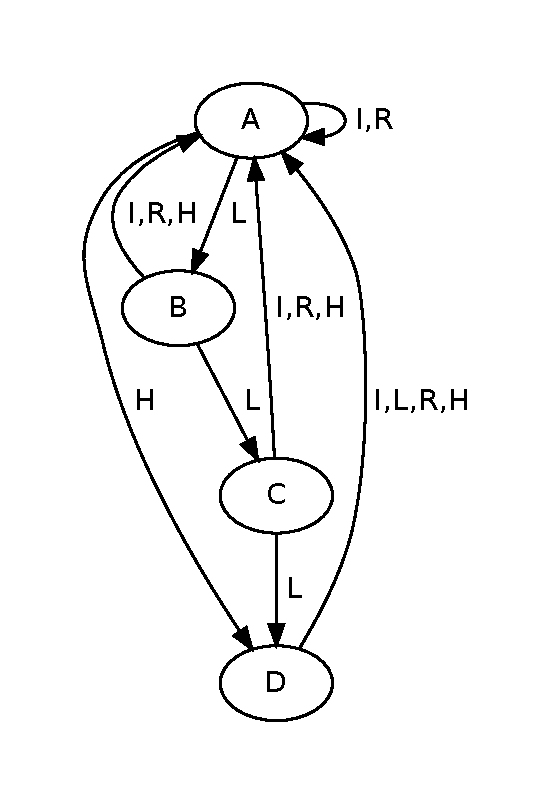
\includegraphics[scale=0.7]{figures/left-signal}
\end{center}
\caption{State diagram for left turn signal operation.
State A has zero lights on (000), state B has one (001),
state C has two (011) and state D has all three (111).
Each transition is denoted with I as idle, R as right, L as left,
and H as hazard.}
\label{fig:leftstate}
\end{figure}

\begin{table}[htbp!]
\center
\begin{tabular}[t]{c|cccc|c}
$S$ &       & $S^+$ &     &     & \\
    & $X=I$ & $L$   & $R$ & $H$ & $Z$ \\
\hline
$A$ & $A$   & $B$   & $A$ & $D$ & 000 \\
$B$ & $A$   & $C$   & $A$ & $A$ & 001 \\
$C$ & $A$   & $D$   & $A$ & $A$ & 011 \\
$D$ & $A$   & $A$   & $A$ & $A$ & 111 \\
\end{tabular}
\caption{State table for LEFT turn signal.
The states of $X$ are all mutually exclusive.}
\label{tbl:leftstate}.
\end{table}

The source code for the Verilog definition of the tail lights
is given in Listing \ref{lst:tl}.
The module is only triggered on the positive edge of the clock (Line 13),
similar to a flip-flop.
The first decision level consists of a chain of \verb+if+ \verb+else+
statements which discriminate among the possible X input values (H, L, R, and
the catch all state I).
For each value the current state of the tail lights (TL, TR) is examined
and a decision is made as to what state to assign next.

\lstinputlisting[
	language=Verilog,
	basicstyle=\footnotesize,
	numbers=left,
	captionpos=b,
	caption={Verilog source for the tail lights.},
	label={lst:tl}
	]{verilog/taillights.v}


% {{{ Compiling Verilog source and running GTKWave
\subsection{Compiling Verilog source and running GTKWave}

Once all the code has been defined it can be compiled and run.
The test bench is given in Appendix\ref{sec:test}.

To compile the source code using Icarus Verilog\cite{VERILOG}
under Linux the following command can be run.

\begin{verbatim}
iverilog test.v
\end{verbatim}

This will produce a filed named 'a.out'.
Under Linux this can be executed directly.

\begin{verbatim}
./a.out
\end{verbatim}

Alternatively the \verb+vvp+ command can be used.
This method works under Linux or Windows.

\begin{verbatim}
vvp a.out
\end{verbatim}

Because the \verb+$dumpfile+ and \verb+$dumpvars+ have been
added to the test bench (Appendix \ref{sec:test})
it will produce an output file suitable for GTKWave\cite{GTKWAVE}.
The file should have the extension '.vcd' and can
be run as shown below.

\begin{verbatim}
gtkwave output.vcd
\end{verbatim}

And from within GTKWave the different variables can be selected
and displayed.

% }}}

% }}}

% {{{ Observations
\section{Observations}

The output for various operations of the turn signal are given
in Figure \ref{fig:waves}.
It can be seen that when it is in either the left or right
position it progresses through the proper tail light sequence.
It also handles transient situations where it is changed from
left to right mid way through a sequence.
And the hazard operation alternates from all on to all off
as it is unaffected by either left or right being actuated at the same time.

\begin{figure}
\center
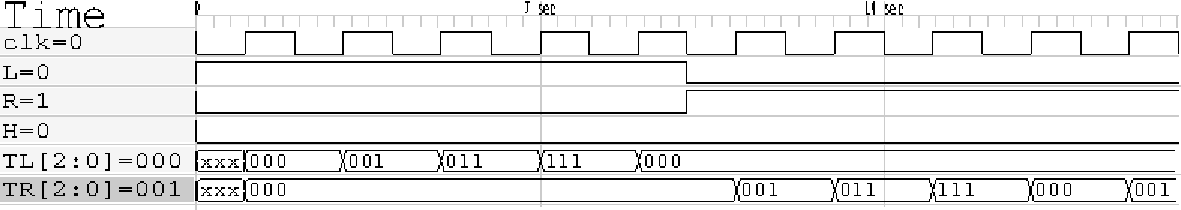
\includegraphics[scale=0.7]{figures/left-right-wave} \\
(a) \\
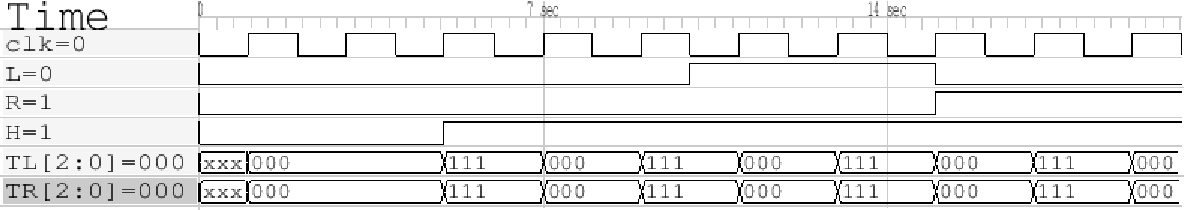
\includegraphics[scale=0.7]{figures/hazard-wave} \\
(b) \\
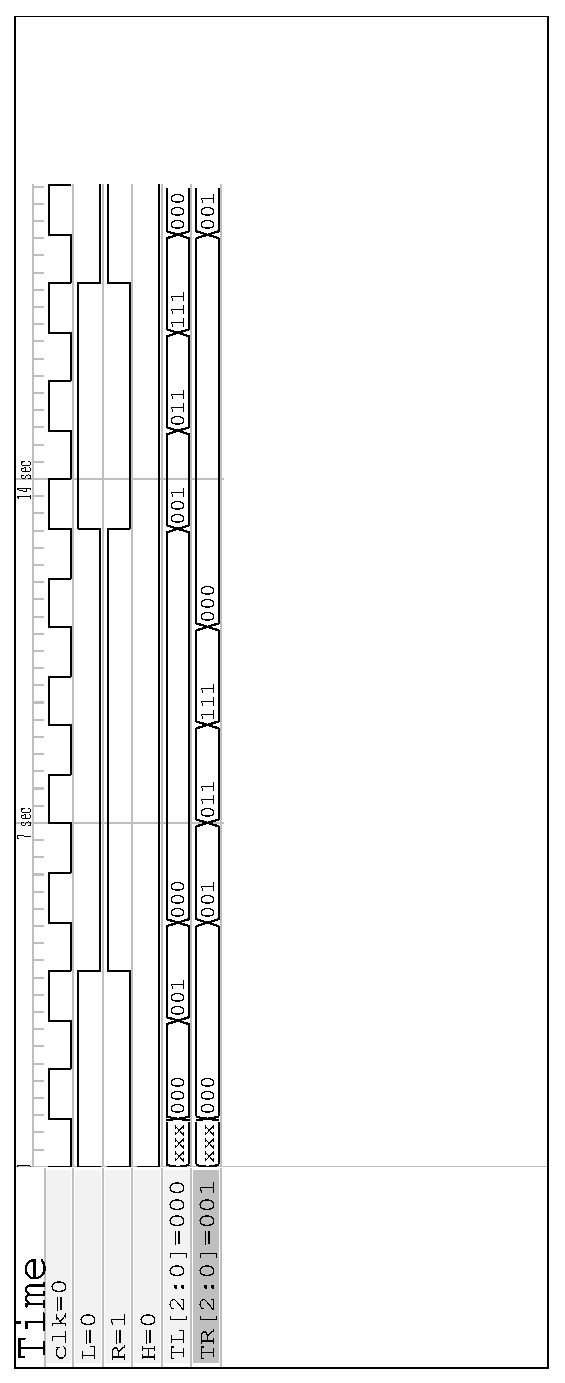
\includegraphics[scale=0.7]{figures/left-right-random-wave} \\
(c)
\caption{Wave forms for of the tail lights in various situations.
In (a) it goes from from left and then switches to right.
In (b) it starts at idle, then the hazards are turned on, then
left turn signal is engaged, and then the right turn signal is engaged.
Notice that the hazard has priority and that the left and right have no effect.
In (c) it is switched back and forth from left to right to show the transitions
when switch midway through a cycle.
}
\label{fig:waves}
\end{figure}

% }}}

% {{{ Conclusion
\section{Conclusion}

This lab was a complete success in implementing a design for
old Thunderbird tail lights in Verilog.
All design requirements were met and the tail lights behaved as
expected.

% }}}

%\clearpage

\renewcommand*{\refname}{\vspace{-8mm}}
\section{References}
%%\bibliographystyle{plain}
%%\bibliographystyle{mslapa}
\bibliographystyle{ieeetr}
\bibliography{../references}

\clearpage
\appendix

\section{Verilog Test Bench}
\label{sec:test}

\lstinputlisting[
	language=Verilog,
	basicstyle=\footnotesize,
	numbers=left
	]{verilog/test.v}

\end{document}

% vim:foldmethod=marker
